\documentclass[11pt,a4paper]{article}

% USEPACKAGE LISTA
\usepackage[utf8]{inputenc}
\usepackage{amsmath}
\usepackage{mathtools}
\usepackage{marvosym} 
\usepackage{wrapfig}
\usepackage{hyperref}
\usepackage{float}
\usepackage{multicol}
\hypersetup{colorlinks,citecolor=black,filecolor=black,linkcolor=black,urlcolor=black}
\usepackage{pdfpages}
\usepackage{amsfonts}
\usepackage{amssymb}
\usepackage{fancyhdr}
\usepackage{graphicx}
\usepackage{t1enc}
\usepackage[magyar]{babel}
\usepackage{bm}
\usepackage{tikz, tcolorbox}
\usepackage{verbatim}

\usepackage{pgfplots}
\pgfplotsset{height = 10cm, width=15cm,compat=1.9}

\usepackage[left=2cm,right=2cm,top=2cm,bottom=2cm]{geometry}

\setlength{\parindent}{0pt}
\setlength{\parskip}{0em}
\pagestyle{fancy}
\fancyhf{}

\title{Matematika G1-G2-G3 kidolgozott tételek}
\author{Kun László Ákos}
\date{2022/2023}

\lhead{2022/2023}
\chead{Matematika Szigorlat tételek}
\rhead{Kun L.}
\cfoot{\thepage. oldal}

% ITT KEZDŐDIK A DOKUMENTUM
\begin{document}

\maketitle{}
\begin{tcolorbox}[colback=green!5!white,colframe=green!60!black,title= MINTA!!]
    \begin{itemize}
        \item To be continued
    \end{itemize}
\end{tcolorbox}
\begin{tcolorbox}[colback=blue!5!white,colframe=blue!70!black,title= MINTA!!]
    \begin{itemize}
        \item To be continued
    \end{itemize}
\end{tcolorbox}
\begin{tcolorbox}[colback=red!5!white,colframe=red!60!black,title= MINTA!!]
    \begin{itemize}
        \item To be continued
    \end{itemize}
\end{tcolorbox}

\newpage
\begin{center}
    \textbf{Matematika G1 szóbeli tételek}
\end{center}
\textbf{Halmazelmélet és komplex számok:}

\begin{tcolorbox}[colback=green!5!white,colframe=green!60!black,title= 1. Halmaz{,} unió{,} metszet{,} különbség]
    \textbf{Halmaz:} Közös tulajdonságú elemek összessége.\\\\
    \textbf{Unió:} Két vagy több halmaz uniója mindazon elemek halmaza, amelyek legalább az egyik halmaznak elemei.
                $$A \cup  B = \{ x \in X\mid x \in A \vee  x \in B\}$$
    \textbf{Metszet:} Két vagy több halmaz metszete pontosan azoknak az elemeknek a halmaza, melyek mindegyik halmaznak elemei
                $$A \cap   B = \{ x \in X\mid x \in A \wedge x \in B\}$$
    \textbf{Különbség:} \(A\) és \(B\) halmaz különbsége az \(A\) halmaz mindazon elemeinek halmaza, amelyek a \(B\) halmaznak nem elemei
                $$A \setminus   B = \{ x \in X\mid x \in A \wedge x \ni B\}$$
    \begin{center}
        \fbox{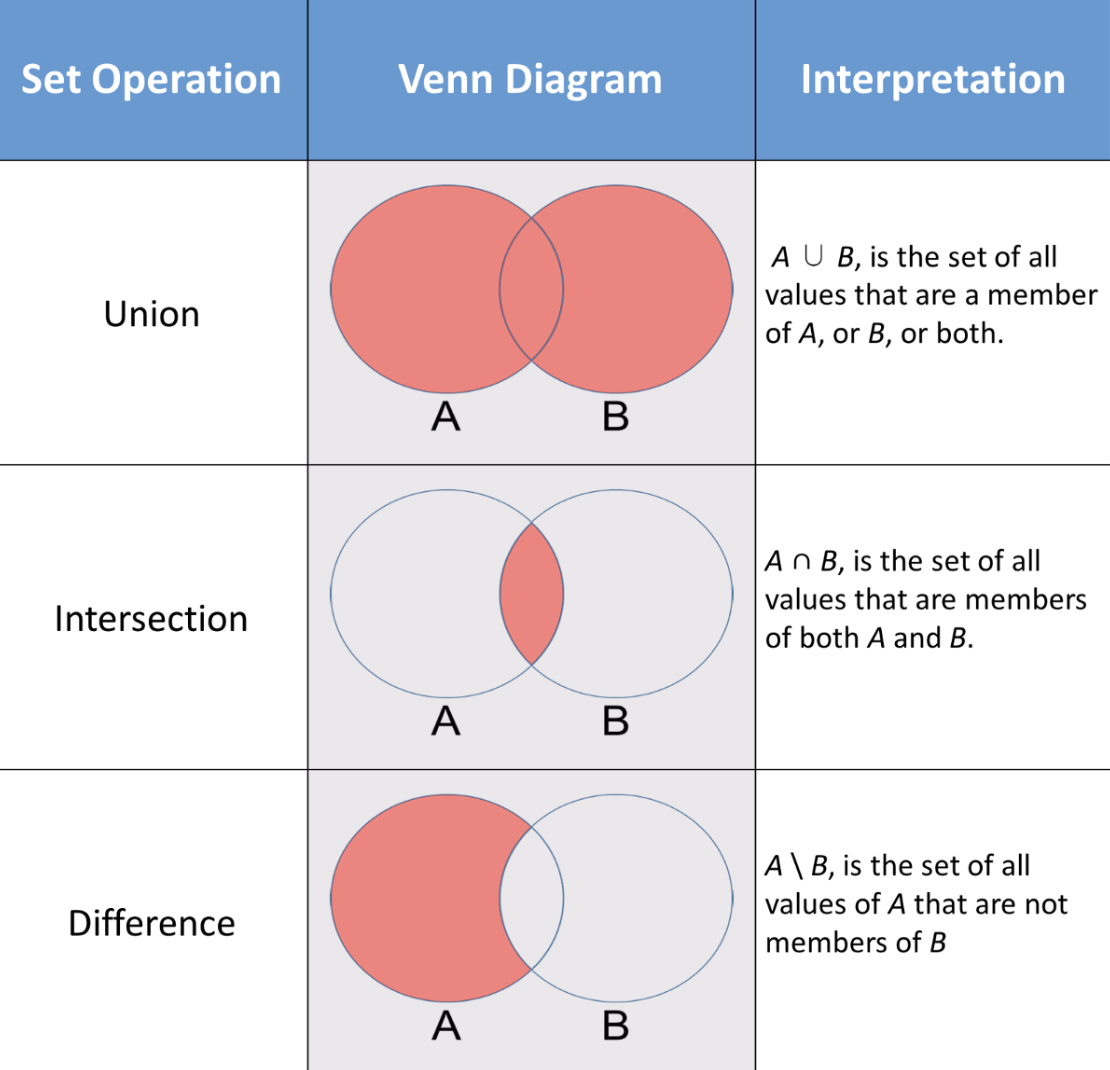
\includegraphics[scale = 0.5]{1.png}}
    \end{center}
\end{tcolorbox}

\begin{tcolorbox}[colback=green!5!white,colframe=green!60!black,title= 2. Descartes-szorzat{,} hatványhalmaz]
    Az A és B Halmazok Descartes-szorzatán az A és B Halmazok elemeiből alkotott összes rendezett elempárok halmazát értjük.
    $$A \times B := \{(a,b)\mid a \in A \wedge b \in B\}$$
    \textbf{Hatványhalmaz:} Egy halmaz összes részhalmazainak halmazát a Halmaz hatványhalmazának hívjuk.
\end{tcolorbox}

\begin{tcolorbox}[colback=green!5!white,colframe=green!60!black,title= 3. Csoport{,} gyűrű{,} test]
        \textbf{Félcsoport:} olyan halmaz, melyben a kétváltozós műveletek asszociatívak (pl. természetes számok esetén az összeadás)\\\\
        \textbf{Csoport:} Legyen \(G\neq 0\) és egy \(\circ \) művelet (szorzás). Ekkor \((G, \circ )\) csoport, ha teljesülnek az alábbiak:
        \begin{enumerate}
            \item \((a \circ b) \circ c = a \circ (b \circ c)\) minden \(a, b, c \in G\) esetén
            \item bármely \(e \in G\), hogy \(a \circ e = e \circ a = a\) minden \(a \in G\) esetén (létezik az egységelem, \(e\), amely asszociatív)
            \item minden \(a \in G\) esetén létezik \(a' \in G\), hogy \(a \circ a'=a' \circ a = e\) (létezik inverzelem)
        \end{enumerate}
        \textbf{Ábel-csoport:} olyan halmaz, melyben a kétváltozós műveletek asszociatívak és kommutatívak is ill. létezik a zérus elem és az inverz elem\\\\
        \textbf{Gyűrű:}
        Legyen \(R\neq 0\) és \(+, \circ \) két művelet. Ekkor \((R, +, \circ )\) gyűrű ha teljesülnek az alábbiak:
        \begin{enumerate}
            \item \((R, +)\) Ábel csoportot alkot (Ábel csoport = kommutatív csoport)
            \item A  művelet asszociatív (csoportosítható) \((a \circ b) \circ c = a \circ (b \circ c)\) minden \(a, b, c \in R\) esetén
            \item A \(\circ \) művelet disztributív \(+\)-ra nézve (összekapcsolható) \((a + b) \circ c = a \circ c + b \circ c\) minden \(a, b, c \in R\) esetén
        \end{enumerate}
        \textbf{Test:} 
        Legyen \(T \neq 0\) és \(+, \circ \) két művelet. Ekkor \((T, +, \circ)\) test ha teljesülnek az alábbiak:
        \begin{enumerate}
            \item (T, +) Ábel csoportot alkot
            \item A \(\circ\) művelet legyen asszociatív (csoportosítható) \((a \circ b) \circ c = a \circ (b \circ c)\) minden \(a, b, c \in R\) esetén
            \item A \(\circ\) művelet legyen disztributív azaz \((a + b) \circ c = a \circ c + b \circ c\) minden \(a, b, c \in R\) esetén
            \item Létezik \(e \in G\), hogy \(a \circ e = e \circ a = a\) minden \(a \in T\) esetén (létezik egységelem a második műveletre)
            \item A \(+\) műveletekhez tartozó egységelem kivételével bármely \(a \in G\) esetén létezik \(a' \in G\), hogy \(a \circ a' = a' \circ a = e\) (létezik az inverz elem, kivéve az első művelethez \((+)\) tartozó egységelem
            esetében)
        \end{enumerate}
\end{tcolorbox}

\begin{tcolorbox}[colback=green!5!white,colframe=green!60!black,title= 4. Komplex számok algebrai{,} trigonometrikus{,} exponenciális alakja]
    \begin{itemize}
        \item \textbf{Algebrai alak:} \(z = a + b\cdot i\) (\(z\) valós része \(a\), képzetes része pedig \(b\))
        \begin{itemize}
            \item \textbf{konjugált:} \(\overline{z} = a - b\cdot i\)
            \item \textbf{abszolút érték:} \(\left\lvert z \right\rvert  = \sqrt{a^2+b^2}\) (Pitagorasz-tételből), és mivel: \\ \(z \cdot \overline{z} = (a + b\cdot i)(a - b\cdot i) = a^2 -(b\cdot i)^2=a^2+b^2\), ezért \( \left\lvert z\right\rvert =\sqrt{z \cdot \overline{z} }  \)
        \end{itemize}
        \item \textbf{Trigonometrikus (polár) alak:} \(z = r(cos(\varphi ) + i \cdot sin(\varphi))\), mivel
        $$ cos(\varphi)=\frac{a}{r} $$
        $$ sin(\varphi)=\frac{b}{r} $$
        Tehát \(a = r\cdot cos(\varphi)\) és \(b = r\cdot sin(\varphi)\), innen már egyértelműen következik a trigonometrikus alak az algebraiból \(r\)-t kiemelve \((a = r\cdot cos(\varphi)\) és \(b\cdot i = r \cdot i\cdot sin(\varphi))\)
        \item \textbf{Exponenciális alak:} \(z = r \cdot e^{i\cdot \varphi}\) - ez csak egy szimbólum, rövidítés, ami megkönnyíti a
        számolást a komplex számokkal, lényegében a trigonometrikus alak kicsit rövidebben.
    \end{itemize}
\end{tcolorbox}

\begin{tcolorbox}[colback=green!5!white,colframe=green!60!black,title= 5. Komplex számok hatványozása]
    \textbf{de Moivre-képlet:} 
    $$z^n = [r(cos(\varphi)+i\cdot sin(\varphi))]^n=r^n(cos(n\varphi)+i\cdot sin(n\varphi))$$
    \textbf{Bizonyítás:} Teljes indukció használatával
    \begin{enumerate}
        \item \(n=1\)-re és \(n=2\)-re \textbf{igaz}
        \item indukciós feltétel: \(n = k\)
        \item Ekkor \(z^k= r^k(cos(k\varphi)+i\cdot sin(k\varphi))\)
        \item ha \(n = k + 1\), akkor:
    \end{enumerate}
    $$z^{k+1}=z^k\cdot k = r^k(cos(k\varphi)+i\cdot sin(k\varphi))\cdot r(cos(\varphi) +i\cdot sin(\varphi))$$
    $$=r^{k+1}[cos(k\varphi + \varphi)+ i\cdot sin(k\varphi + \varphi)] =$$
    $$r^{k+1}[cos((k+1)\varphi)+ i\cdot sin((k+1)\varphi)] $$\\
    és \(k+1\) az \(n\) volt, tehát a bizonyítás kész.

\end{tcolorbox}

\begin{tcolorbox}[colback=green!5!white,colframe=green!60!black,title= 6. Komplex számok gyökvonása]
$$z_1^n = z_2=r_1^n\cdot (cos(n\varphi_1)+i\cdot sin(n\varphi_1)) = r_2\cdot (cos(\varphi_2)+i\cdot sin(\varphi_2))$$  
$$z_1 = \sqrt[n]{z_2} $$  
\textbf{Két komplex szám akkor egyenlő, ha a hosszuk és argumentumuk is egyenlő:}
    \begin{itemize}
        \item \(r_1= \sqrt[n]{r_2}\) \hspace{61pt} (\textbf{hossz})
        \item \(n\cdot \varphi_1 = \varphi_2 + k\cdot 2\pi\) \hspace{10pt} (\textbf{argumentum}) \(\rightarrow\) forgásszög, periodicitás miatt \(p = 2\pi \)
        \item Így \(\varphi_1 = \frac{\varphi_2+k\cdot2\pi}{n} \hspace{30pt}\) \(k \in \{0, 1, 2, ... , n - 1\}\)
        \item Tehát: 
    \end{itemize}
    $$\sqrt[n]{z}= \sqrt[n]{r}(cos(\frac{\varphi+k\cdot2\pi}{n}) + i\cdot sin(\frac{\varphi+k\cdot2\pi}{n}))$$
    Az \(n\)-edik gyökvonás után olyan komplex számokat kapunk, amik egy szabályos sokszög
    (\(n\)-szög) csúcsai! Tehát n-edik gyökvonás esetén \(n\) db komplex szám a megoldás.
\end{tcolorbox}
\newpage

\textbf{Numerikus sorozatok:}

\begin{tcolorbox}[colback=green!5!white,colframe=green!60!black,title= 1. Numerikus sorozat határértéke]
Az \((a_n)\) sorozatot konvergens és határértéke az \(a \in R\) akkor és csak akkor, ha bármely \(\varepsilon > 0\) értékhez
létezik olyan \(N(\varepsilon)\) küszöbindex, hogy a sorozat \(N(\varepsilon)\)-nél nagyobb indexű elemei az az \(\varepsilon\) sugarú környezetében vannak.
Az \((a_n)\) sorozatot konvergens és határértéke az \(a \in R\) akkor és csak akkor, ha bármely \(\varepsilon > 0\) sugarú
környezetén kívül a sorozatnak csak véges sok eleme van.
\end{tcolorbox}

\begin{tcolorbox}[colback=green!5!white,colframe=green!60!black,title= 2. Konvergens{,} divergens sorozat]
    \begin{itemize}
        \item \textbf{Definíció:} Az \((a_n)\) konvergens, ha van olyan \(a \in R\) szám, hogy minden \(\varepsilon > 0\) valós szám esetén létezik \(N(\varepsilon)\) valós küszöbszám, hogy
    \end{itemize}
        $$\left\lvert a_n -a\right\rvert < \varepsilon,\hspace{5pt}ha\hspace{5pt}n > N(\varepsilon)$$
    \begin{itemize}
        \item Az \("a"\) számot az \((a_n)\) határértékének hívjuk, és a \(\lim_{n \to \infty} a_n = a\)  vagy az \(a_n \to a\), ha \(n \to \infty \) jelölést használjuk.
        \item Az \((a_n)\) divergens, ha nem konvergens.
    \end{itemize}
\textbf{Tételek:}
\begin{itemize}
    \item Konvergens sorozat korlátos.
    \item Monoton korlátos sorozat konvergens.
    \item van határértéke/torlódási pontjai \(\rightarrow\) nem biztos, hogy konvergens
    \item \textbf{Bolzano-Weierstrass-tétel:} minden korlátos sorozatnak van konvergens részsorozata.
\end{itemize}
\end{tcolorbox}

\begin{tcolorbox}[colback=green!5!white,colframe=green!60!black,title= 3. Nevezetes sorozatok]
    Olyan sorozatok, amelyek határértékét nem kell bizonyítani, csak felhasználni!\\\\
    \textbf{Bernoulli-féle egyenlőtlenség:} ha \(x \geq  -1\), akkor \((1+x)^n \geq 1 + n\cdot x\)
    \begin{enumerate}
        \item \(a^n \to 0\), ha \(\left\lvert a\right\rvert <1\)\\
        \(a^n \to 1\), ha \(a=1\)\\
        \(a^n \to +\infty\), ha \(a>1\)\\
        \(a^n\) divergens, ha \(a<-1\)
        \item \(\sqrt[n]{a} \to 1\), ha \(n \to \infty (a>0)\)
        \item \(a^n\cdot n^k \rightarrow 0\), nullsorozat, ha \(\left\lvert a\right\rvert <1 \) és \(k\) rögzített természetes szám
        \item \(\sqrt[n]{n} \to 1\), ha \(n \to \infty \hspace{5pt}(n\geq 2)\)
        \item \(\frac{a^n}{n!} \to 0 (a \in \mathbb{R} )\)
    \end{enumerate}
    \textbf{Legfontosabb:}
    $$(1+\frac{\alpha}{n})^n \to e^{\alpha}$$
\end{tcolorbox}

\begin{tcolorbox}[colback=green!5!white,colframe=green!60!black,title= 4. Cauchy sorozat]
        \textbf{Definíció:} Az \((a_n)\)-t Cauchy-sorozatnak nevezzük, ha minden \(\varepsilon > 0\) esetén \(\exists N(\varepsilon)\) küszöbindex, hogy: 
        \begin{center}
            \(\left\lvert a_n -a_m\right\rvert  < \varepsilon\), ha \(n,m > N(\varepsilon)\) \(\hspace{15pt}\) \((n,m \in N)\)
        \end{center}
        \textbf{Tétel:} Cauchy-féle konvergencia kritérium (szükséges és elégséges feltétel). Az \((a_n)\) akkor és csak akkor konvergens, ha Cauchy sorozat!
\end{tcolorbox}

\begin{tcolorbox}[colback=green!5!white,colframe=green!60!black,title= 5. Torlódási pont]
        \textbf{Definíció:} A \(h\) a \(H\) halmaz torlódási pontja, ha \(h\) bármely környezetében van \(H\)-nak \(h\)-tól
        különböző eleme. A \(t\) szám a sorozat torlódási pontja, ha \(t\) akármilyen kicsi környezete a sorozat végtelen sok
        elemét tartalmazza. Például: \((-1)^n\)
\end{tcolorbox}
\newpage

\textbf{Függvények, derivált:}

\begin{tcolorbox}[colback=green!5!white,colframe=green!60!black,title= 1. Függvények{,} értelmezési tartomány{,} értékkészlet]
        \textbf{Függvény:} ha az \(A\) (nemüres) halmaz minden egyes eleméhez hozzárendeljük a \(B\)
        (nemüres) halmaz pontosan egy elemét, akkor ezt a leképezést függvénynek nevezzük.
        $$f:A \to B$$
        \textbf{Értelmezési tartomány:} azon elemek halmaza, melyekhez a függvény hozzárendel
        egy-egy elemet a B halmazból, jelen esetben ez az A halmaz.
        $$D_f = A$$
        \textbf{Értékkészlet:} A képhalmaz, azaz a \(B\) halmaz azon elemei, melyeket az \(f\) függvény
        ténylegesen hozzárendel az \(A\) valamelyik eleméhez. Az értékkészlet tehát része a képhalmaznak:
        $$R_f \subset B$$
\end{tcolorbox}

\begin{tcolorbox}[colback=green!5!white,colframe=green!60!black,title= 2. Függvény határérték]
Azt mondjuk, hogy az \(f\) függvény határértéke az \("a"\) pontban \(A\), ha minden \(\varepsilon > 0\) számhoz
létezik olyan \(\delta(\varepsilon)  > 0\), hogy ha \(0 < \left\lvert x-a \right\rvert  < \delta(\varepsilon)\), akkor \(|f(x) - A| < \varepsilon\).\\
/Ez a Cauchy-féle definíció/\\
\begin{center}
    \(|x - a| < \delta(\varepsilon)\) azt jelenti, hogy:
\end{center}
    $$- \delta(\varepsilon) < x - a < \delta(\varepsilon) \hspace{10pt} /+a$$
    $$a - \delta(\varepsilon) < x < a + \delta(\varepsilon)$$

\textbf{Szemléletesesen:} azt jelenti, hogy a függvényértékek \((f(x)-ek)\) tetszőlegesen megközelítik az
A számot, ha az \(\varepsilon\) értékek elég közel kerülnek \(a\)-hoz. Az \(f\) függvénynek az \("a"\) pontban acsa (akkor és csak akkor) van határértéke, ha van bal- és
jobboldali határértéke és ez a kettő megegyezik!
\begin{itemize}
    \item \textbf{Határérték a végtelenben:}
    \begin{itemize}
        \item Az \(f\) függvény határértéke \(+\infty\)-ben \(A\), ha minden \(\varepsilon > 0\) esetén van olyan \(N(\varepsilon)\), hogy
    \(|f(x) - A| < \varepsilon\), ha \(x > N(\varepsilon)\).
        \item Az \(f\) függvény határértéke \(-\infty\)-ben \(A\), ha minden \(\varepsilon > 0\) esetén van olyan \(N(\varepsilon)\), hogy
    \(|f(x) - A| < \varepsilon\), ha \(x < N(\varepsilon)\).
    \end{itemize}
    \item \textbf{A végtelen, mint határérték:}
    \begin{itemize}
        \item Az \(f\) függvény határértéke \(a\)-ban \(+ \infty\), ha bármely \(N > 0\) esetén van olyan \(\delta(N)\), hogy \(f(x) > N\), ha \(0 < |x - a| < \delta(N)\).
        \item Az \(f\) függvény határértéke \(a\)-ban \(- \infty\), ha bármely \(N > 0\) esetén van olyan \(\delta(N)\), hogy \(f(x) < N\), ha \(0 < |x - a| < \delta(N)\).
    \end{itemize}
\end{itemize}
\end{tcolorbox}

\begin{tcolorbox}[colback=green!5!white,colframe=green!60!black,title= 3. Függvény folytonosság]
    Az \(f\) függvény az értelmezési tartományának \("a"\) pontjában folytonos, ha ebben a pontban
létezik határértéke és ez egyenlő az adott pontbeli helyettesítési értékkel, azaz ha
$$\lim_{x \to a} f(x) = f(a) $$
    \begin{itemize}
        \item \textbf{Definíció:} Az \(f\) függvényt folytonosnak nevezzük az \(a \in D_f\) pontban, ha bármely \(\varepsilon > 0\)
        esetén van olyan \(\delta(\varepsilon) > 0\) szám, hogy ha \(|x - a| < \delta(\varepsilon)\), akkor \(|f(x) - f(a)| < \varepsilon\).
    \end{itemize}
    Az \(f\) függvény egy intervallumon egyenletesen folytonos, ha bármely \(\varepsilon > 0\) számhoz van
    olyan \(\delta > 0\) szám, hogy \(f\) értelmezési tartományának bármely \(x_1\), \(x_2\) elemére, amelyek
    távolsága egymástól kisebb \(\delta\)-nál, fennáll az alábbi egyenlőtlenség.
    $$|f(x_1) - f(x_2)| < \varepsilon$$
    \begin{itemize}
        \item \textbf{Tétel:} Az \(f\) függvény pontosan akkor folytonos értelmezési tartományának \("a"\) pontjában, ha
        ott balról és jobbról is folytonos.
        \item \textbf{Definíció:} Az \(f\) függvény folytonos az \( ] a, b [ \)-on, ha folytonos \(]a, b[ \) minden pontjában.
        Az f függvény folytonos az \([a, b]\)-on, ha folytonos \(]a, b[\)-on és \(a\)-ban balról, \(b\)-ben
        jobbról folytonos.
    \end{itemize}
    \textbf{A folytonosság néhány nevezetes következménye:}\\
        Ha \(f\) folytonos egy zárt intervallumon, akkor ott egyenletesen folytonos.\\\\
        \textbf{Bolzano-tétel:} ha a függvény a zárt intervallumon folytonos, és az intervallum két
        végpontjában az értékei különböző előjelűek, akkor az intervallum belsejében van
        zérushelye. Másképp: felvesz minden \(f(a)\) és \(f(b)\) közé eső értéket egy folytonos függvény egy zárt intervallumon.\\\\
        \textbf{Weierstrass-tétel:} Zárt intervallumon folytonos függvény felveszi a minimumát és a
        maximumát is függvényértékként; továbbá minden olyan értéket, ami a legnagyobb és
        legkisebb érték közé esik.

\end{tcolorbox}

\begin{tcolorbox}[colback=green!5!white,colframe=green!60!black,title= 4. Inverz függvény]
Ha az \(f:X \to Y\) függvénynél a leképezés irányát megfordítjuk, vagyis az \(Y\) halmaz elemeit
képezzük le az \(X\) halmaz elemeire, akkor ez a fordított leképezés általában nem függvény, mert nem biztos, hogy egy \(y \in Y\) elemnek egyetlen \(x \in X\) elem felel meg. Ezért fontos az, hogy f bijektív, azaz kölcsönösen egyértelmű legyen, mert ekkor az \(f-1\) -gyel jelölt fordított leképezés is már függvény lesz.    
    \begin{itemize}
        \item \textbf{Definíció:} Ha az \(f: X \to Y\) függvény kölcsönösen egyértelmű, akkor az \(f^{-1} = Y \to X\)
        függvényt \(f\) inverz függvényének nevezzük. Ekkor igaz az alábbi összefüggés:
    \end{itemize}
    $$f^{-1}(f(x)) = f(f^{-1}(x)) = x$$
\end{tcolorbox}

\begin{tcolorbox}[colback=green!5!white,colframe=green!60!black,title= 5. Derivált]
Ha létezik és véges az alábbi differenciálhányados határértéke:\\
$$Lim_{x\to a}\frac{f(x)-f(a)}{x-a}$$ \\
akkor azt az \(f\) függvény deriváltjának vagy \("a"\) pontbeli differenciálhányadosának nevezzük.\\ 
\textbf{Jelölés:} $$\frac{d f(a)}{d x} = f'(a)$$
\end{tcolorbox}

\begin{tcolorbox}[colback=green!5!white,colframe=green!60!black,title= 6. Lokális szélsőérték definíciója és feltétele]
Legyen \(f : I \subset  R \to R\); \(a\subset  I\)\\
    Azt mondjuk, hogy \(f\) függvénynek a pontban lokális maximuma van, ha létezik \(\delta > 0\), hogy:
    $$f(x) \leq  f(a) (\forall  x \in K)$$
    Azt mondjuk, hogy \(f\) függvénynek a pontban lokális minimuma van, ha létezik \(\delta > 0\), hogy:
    $$f(x) \geq  f(a) (\forall  x \in K)$$
    \textbf{Szükséges feltétel:}\\
    Ha \(f : I \subset  R \to R\) differenciálható függvény és \(f\)-nek  \(\alpha \in int.\hspace{5pt}I-ben\) (\(I\) belseje) szélsőértéke van, akkor\(f'(\alpha)=0\)\\\\
    \textbf{Elégséges feltétel:}\\
    Ha \(f : I \subset  R \to R\) differenciálható függvény és \(\alpha \in int. \hspace{5pt}I\) továbbá létezik \(r > 0\), és teljesül az alábbi
feltétel, akkor \(f\)-nek \(\alpha\)-ban lokális minimuma van.\\
$$f'(x) \leq 0 \to x\in](\alpha -r); \alpha[$$
$$f'(x) \geq 0 \to x\in]\alpha; (\alpha + r)[$$
    Ha \(f : I \subset  R \to R\) differenciálható függvény és \(\alpha \in int. \hspace{5pt}I\) továbbá létezik \(r > 0\), és teljesül az alábbi
feltétel, akkor \(f\)-nek \(\alpha\)-ban lokális maximuma van.
$$f'(x) \geq 0 \to x\in](\alpha -r); \alpha[$$
$$f'(x) \leq 0 \to x\in]\alpha; (\alpha + r)[$$

\end{tcolorbox}

\begin{tcolorbox}[colback=green!5!white,colframe=green!60!black,title= 7. L'Hôpital szabály]
    Legyen \(f\) és \(g\) differenciálható függvények az \(\alpha\) pont egy környezetében, továbbá:
    \begin{center}
        \(Lim_{x \to \alpha} f(x)=Lim_{x \to \alpha} g(x)=0\) \hspace{10pt} vagy \hspace{10pt} \(\left\lvert Lim_{x \to \alpha} f(x) \right\rvert = \left\lvert Lim_{x \to \alpha} g(x) \right\rvert = \infty  \)\\
        \(\alpha \in \{0; \pm \infty \}\)
    \end{center}
    Ekkor: 
    $$\frac{Lim_{x \to \alpha} f'(x)}{Lim_{x \to \alpha} g'(x)} = \frac{Lim_{x \to \alpha} f(x)}{Lim_{x \to \alpha} f(x)} $$
\end{tcolorbox}
\newpage
\textbf{Középérték tételek és Integrálás:}

\begin{tcolorbox}[colback=green!5!white,colframe=green!60!black,title= 1. Lagrange középérték tétel]
    Legyen \(f : I \subset R \to R\) folytonos \([a; b]\) intervallumon és differenciálható \(]a; b[\) intervallumon. Ekkor
létezik olyan \(\delta \in ]a; b[\) hogy:
$$f'(\delta) = \frac{f(b)-f(a)}{b-a}$$
\end{tcolorbox}

\begin{tcolorbox}[colback=green!5!white,colframe=green!60!black,title= 2. Rolle középérték tétel]
    Legyen \(f\) folytonos \([a; b]\) intervallumon és differenciálható \(]a; b[\) intervallumon, továbbá \(f(a) = f(b) = 0\)
Ekkor létezik \( \xi \in ]a; b[\) melyre teljesül, hogy:
$$f'(\xi) = 0$$
\end{tcolorbox}

\begin{tcolorbox}[colback=green!5!white,colframe=green!60!black,title= 3. Cauchy középérték tétel]
    Legyen \(f\) és \(g\) függvények folytonosak \([a; b]\) intervallumon és differenciálhatóak \(]a; b[\) intervallumon,
valamint tegyük fel, hogy \(g'(x) \neq 0\) bármely \(x \in ]a; b[\) esetén. Ekkor létezik olyan \(\delta \in]a; b[\) hogy:
$$\frac{f(b)-f(a)}{g(b)-g(a)} = \frac{f'(\delta)}{g'(\delta)}$$
\end{tcolorbox}

\begin{tcolorbox}[colback=green!5!white,colframe=green!60!black,title= 4. Riemann-Integrálhatóság]
    Az \(f\) függvény Riemann-integrálható \([a; b]\) intervallumon, ha a Darboux-féle alsó- és felső-integrálja
megegyezik. Ezt a közös értéket az \(f\) függvény Riemann-integráljának nevezzük.
\end{tcolorbox}

\begin{tcolorbox}[colback=green!5!white,colframe=green!60!black,title= 5. Newton-Leibniz formula]
    Legyen \(f\) függvény Riemann-integrálható \([a; b]\) intervallumon és \(F : [a; b] \to \mathbb{R} \) olyan primitív függvény,
hogy \(F\) folytonos \([a; b]\) intervallumon, \(F\) differenciálható \(]a; b[\) intervallumon és \(F'(x) = f(x)\) bármely
\(x \in ]a; b[\) Ekkor:
$$\int_{a}^{b} f = F(b)-F(a) $$
\end{tcolorbox}

\begin{tcolorbox}[colback=green!5!white,colframe=green!60!black,title= 6. Improprius integrál]
    Legyen \((a; b) \in \mathbb{R}_b \) és \((a < b)\) valamint
    \begin{enumerate}
        \item minden \([x; y] \subset  ]a; b[\) esetén \(f\) Riemann-int. \([x; y]\) intervallumon és \((x; y) \subset \mathbb{R}\)
        \item létezik olyan \(c \in \mathbb{R}  (a < c < b)\), hogy az alábbi határértékek léteznek és végesek:
    \end{enumerate}
    \begin{center}
        \(Lim_{x \to \alpha }\int_{x}^{c} f(t) \,dt\) \(\hspace{15pt}\) és \(\hspace{15pt}\) \(Lim_{y \to b }\int_{c}^{y} f(t) \,dt\)
    \end{center}
    Ekkor az \(I:= Lim_{x \to \alpha }\int_{x}^{c} f(t) \,dt +  Lim_{y \to b }\int_{c}^{y} f(t) \,dt \) összeget az \(f\) függvény improprius integráljának nevezzük \(]a; b[\) intervallumon és \(\int_{a}^{b} f(b) \,dt \) jelöljük.\\\\
    Azt is mondjuk, hogy az \(f\) függvény improprius Riemann-integrálja az \(]a; b[\) intervallumon konvergens.
Ha az 1. feltétel teljesül, de a 2. feltétel nem, akkor az \(f\) függvény improprius Riemann-integrálja
divergens.
\end{tcolorbox}

\newpage
\textbf{Numerikus sorok:}

\begin{tcolorbox}[colback=green!5!white,colframe=green!60!black,title= 1. Numerikus sor fogalma]
    Az \(a_n\) numerikus sorozat tagjaiból képzett végtelen összeget numerikus sornak nevezzük. Jelölése:
    $$\sum_{n = 1}^{\infty} a_n $$
\end{tcolorbox}

\begin{tcolorbox}[colback=green!5!white,colframe=green!60!black,title= 2. Numerikus sor konvergenciája]
A \(\sum_{n = 1}^{\infty} a_n\) numerikus sor konvergens, akkor és csak akkor, ha bármely \(\varepsilon\) > 0 esetén létezik olyan \(N(\varepsilon)\)
hogy:
$$\left\lvert a_{n+1} + a_{n+2} + ... + a_m\right\rvert < \varepsilon \hspace{40pt} (n, m >N_{(\varepsilon)}$$

\textbf{Feltételes konvergencia:}\\
Ha \(\sum a_n\) sor konvergens, de nem abszolút konvergens (abszolút konvergens, ha \(\sum \left\lvert a_n\right\rvert \)  konvergens), akkor feltételes konvergenciáról beszélünk.
\end{tcolorbox}

\begin{tcolorbox}[colback=green!5!white,colframe=green!60!black,title= 3. Numerikus sor divergenciája]
    Ha a numerikus sor nem konvergens, akkor divergens.
\end{tcolorbox}

\begin{tcolorbox}[colback=green!5!white,colframe=green!60!black,title= 4. Konvergencia tesztek]
    \begin{itemize}
        \item \textbf{Majorálás/minorálás:}\\
        Legyen \(\sum a_n\) és \(\sum b_n\) nemnegatív tagú sorok, melyekre teljesül az hogy \(a_n < b_n\) bármely \(n \in N\)
        esetén, ekkor:
        \begin{itemize}
        \item \textbf{Minorálás:} Ha \(\sum a_n\) divergens, akkor \(\sum b_n\) is az
        \item \textbf{Majorálás:} Ha \(\sum b_n\) konvergens, akkor \(\sum a_n\) is az
        \end{itemize}
    \end{itemize}
    \begin{itemize}
        \item \textbf{D'Alambert-féle hányadosteszt:}\\
        Legyen \(\sum a_n\) egy pozitív tagú sor, ha létezik olyan \(0 < q < 1\) valós szám, amelyre az \(n \in N\) feltétel
mellett az alábbi egyenlet teljesül, akkor konvergens:
    \end{itemize}
    $$\frac{a_n +1}{a_n} < q$$
    \begin{itemize}
        \item \textbf{Cauchy-féle gyökteszt:}\\
        Legyen \(\sum a_n\) egy nemnegatív tagú sor, ha létezik olyan \(0 < q < 1\) valós szám, amelyre az \(n \in N\)
feltétel mellett az alábbi egyenlet teljesül, akkor konvergens:
    \end{itemize}
    $$\sqrt[n]{a_n} < q$$
\end{tcolorbox}

\newpage
\begin{center}
    \textbf{Matematika G2 szóbeli tételek}
\end{center}
\textbf{Lineáris algebra I:}
\begin{tcolorbox}[colback=blue!5!white,colframe=blue!70!black,title= 1. Csoport{,} gyűrű{,} test]
    \textbf{Félcsoport:} olyan halmaz, melyben a kétváltozós műveletek asszociatívak (pl. természetes számok esetén az összeadás)\\\\
        \textbf{Csoport:} Legyen \(G\neq 0\) és egy \(\circ \) művelet (szorzás). Ekkor \((G, \circ )\) csoport, ha teljesülnek az alábbiak:
        \begin{enumerate}
            \item \((a \circ b) \circ c = a \circ (b \circ c)\) minden \(a, b, c \in G\) esetén
            \item bármely \(e \in G\), hogy \(a \circ e = e \circ a = a\) minden \(a \in G\) esetén (létezik az egységelem, \(e\), amely asszociatív)
            \item minden \(a \in G\) esetén létezik \(a' \in G\), hogy \(a \circ a'=a' \circ a = e\) (létezik inverzelem)
        \end{enumerate}
        \textbf{Ábel-csoport:} olyan halmaz, melyben a kétváltozós műveletek asszociatívak és kommutatívak is ill. létezik a zérus elem és az inverz elem\\\\
        \textbf{Gyűrű:}
        Legyen \(R\neq 0\) és \(+, \circ \) két művelet. Ekkor \((R, +, \circ )\) gyűrű ha teljesülnek az alábbiak:
        \begin{enumerate}
            \item \((R, +)\) Ábel csoportot alkot (Ábel csoport = kommutatív csoport)
            \item A  művelet asszociatív (csoportosítható) \((a \circ b) \circ c = a \circ (b \circ c)\) minden \(a, b, c \in R\) esetén
            \item A \(\circ \) művelet disztributív \(+\)-ra nézve (összekapcsolható) \((a + b) \circ c = a \circ c + b \circ c\) minden \(a, b, c \in R\) esetén
        \end{enumerate}
        \textbf{Test:} 
        Legyen \(T \neq 0\) és \(+, \circ \) két művelet. Ekkor \((T, +, \circ)\) test ha teljesülnek az alábbiak:
        \begin{enumerate}
            \item (T, +) Ábel csoportot alkot
            \item A \(\circ\) művelet legyen asszociatív (csoportosítható) \((a \circ b) \circ c = a \circ (b \circ c)\) minden \(a, b, c \in R\) esetén
            \item A \(\circ\) művelet legyen disztributív azaz \((a + b) \circ c = a \circ c + b \circ c\) minden \(a, b, c \in R\) esetén
            \item Létezik \(e \in G\), hogy \(a \circ e = e \circ a = a\) minden \(a \in T\) esetén (létezik egységelem a második műveletre)
            \item A \(+\) műveletekhez tartozó egységelem kivételével bármely \(a \in G\) esetén létezik \(a' \in G\), hogy \(a \circ a' = a' \circ a = e\) (létezik az inverz elem, kivéve az első művelethez \((+)\) tartozó egységelem
            esetében)
        \end{enumerate}
\end{tcolorbox}

\begin{tcolorbox}[colback=blue!5!white,colframe=blue!70!black,title= 2. Euklideszi tér]
Euklideszi térnek nevezzük azon \(T\) számtest feletti vektortereket, amelyekben a verktorterek axiómái értelmezve vannak, valamint az ún. skaláris szorzást:    
    \begin{enumerate}
        \item A skaláris szorzat \(V\)-beli rendezett párokhoz egy \(T\)-beli nemnegatív elemet rendelő függvény, vagyis:
        $$\forall \underline{a},\underline{b} \in V,<\underline{a},\underline{b}>:V \times V \to T$$
        \item a skaláris szorzat kommutatív:
        $$\forall \underline{a}, \underline{b} \in V, <\underline{a}, \underline{b} > =<\underline{b}, \underline{a} >$$
        \item A skalárszorzás kiemelhető:
        $$\forall \underline {a},\underline{b} \in V, \lambda \in T, <\lambda \underline{a}, \underline{b} > = \lambda <\underline{a}, \underline{b}>$$
        \item Az összeg asszociatív:
        $$\forall \underline{a}, \underline{b}, \underline{c} \in V, <\underline{a} + \underline{b},\underline{c}> = <\underline{a}, \underline{c}> + <\underline{b}, \underline{c}>$$
    \end{enumerate}
\end{tcolorbox}

\begin{tcolorbox}[colback=blue!5!white,colframe=blue!70!black,title= 3. Vektortér]
    Legyen \(V\) nem üres halmaz, \(+, \circ \) műveletek, \(T\) test. \((V, +, \circ)\) \(T\) test feletti vektortér, ha:
    \begin{enumerate}
        \item \((V, +)\) Ábel-csoport
        \item valamint:
        \begin{center}
        \(\forall \alpha, \beta \in T,\) és \(\underline{x} \in V : (\alpha \circ \beta) \circ \underline{x} = a\circ (\beta \circ \underline{x})\)
        \end{center}
        \item Ha \(\epsilon\)  a \(T\)-beli egység, akkor:
        $$\forall \underline{x} \in V: \epsilon \circ \underline{x} = \underline{x}$$
        \begin{center}
            \(\forall \alpha, \beta \in T \) és \(\underline{x},\underline{y} \in V: (\alpha +\beta) \circ \underline{x} = \alpha \circ \underline{x} + \beta \circ \underline{x}\) (rendes \(+\))
        \end{center}
        valamint: 
        \begin{center}
            \(\alpha \circ (\underline{x}+\underline{y}) = \alpha \circ \underline{x} + \alpha \circ \underline{y}\) (\(V\)-beli \(+\))
        \end{center}
    \end{enumerate}
\end{tcolorbox}

\begin{tcolorbox}[colback=blue!5!white,colframe=blue!70!black,title= 4. Vektorok lineáris függősége és függetlensége]
    \(\{ b_1, b_2, ..., b_n\}\) vektor lineárisan független, amennyiben az alábbi egyenletnek csak a triviális megoldása létezik, ellenkező esetben lineárisan függő:
    $$\lambda_1 \underline{b_1} +...+\lambda_n \underline{b_n}$$
\end{tcolorbox}

\end{document}